\begin{center}
Problema A

Caminho da Colheita

{\small Nome do arquivo: A.c, A.cpp, A.java, ou A.py}

{\large Timelimit: $1$}

{\tiny Por Athos José}

\end{center}

Seu Zé, fazendeiro importante de Rio Verde tem uma plantação de abóboras organizadas em uma área retangular de tamanho $N$ x $M$, cada muda de abóbora está em uma área $1$x$1$ e contém uma certa quantidade de abóboras.

Costumeiramente, Seu Zé faz a colheita em um percurso único, começando no canto superior esquerdo do campo (posição ($1,1$)) e termina sempre no canto inferior direito do campo ($N,M$). A cada passo, ele mover-se apenas para a direita ou para baixo.

A plantação de Seu Zé cresceu muito e acredita que o carinho que usa para colher não é suficientemente grande para acomodar todas as abóboras no caminho. Agora ele pediu sua ajuda para que dado o campo informa-se qual é máximo de abóboras possível de colher ao longo do melhor caminho.

\vspace{0.3cm}
\begin{figure}[h]
    \centering
    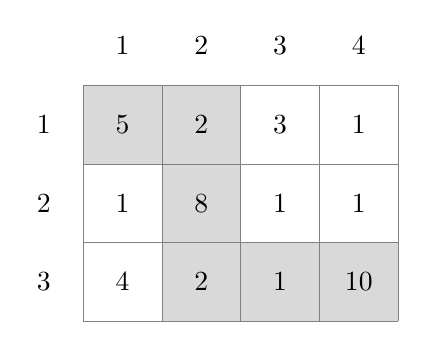
\begin{tikzpicture}
        \fill[gray!30] (0,2) rectangle (1,3);
        \fill[gray!30] (1,2) rectangle (2,3);
        \fill[gray!30] (1,1) rectangle (2,2);
        \fill[gray!30] (1,0) rectangle (2,1);
        \fill[gray!30] (2,0) rectangle (3,1);
        \fill[gray!30] (3,0) rectangle (4,1);

        \draw[gray,very thin] (0,0) grid (4, 3);

        \node at (0.5, 2.5) {5};
        \node at (1.5, 2.5) {2};
        \node at (2.5, 2.5) {3};
        \node at (3.5, 2.5) {1};

        \node at (0.5, 1.5) {1};
        \node at (1.5, 1.5) {8};
        \node at (2.5, 1.5) {1};
        \node at (3.5, 1.5) {1};

        \node at (0.5, 0.5) {4};
        \node at (1.5, 0.5) {2};
        \node at (2.5, 0.5) {1};
        \node at (3.5, 0.5) {10};

        \node at (1.5, 3.5) {2};
        \node at (0.5, 3.5) {1};
        \node at (2.5, 3.5) {3};
        \node at (3.5, 3.5) {4};

        \node at (-0.5, 2.5) {1};
        \node at (-0.5, 1.5) {2};
        \node at (-0.5, 0.5) {3};
    \end{tikzpicture}
    \caption{Exemplo da entrada com células coloridas}
\end{figure}

\vspace{0.3cm}
\textbf{Entrada}

A primeira linha contém dois inteiros $N$ e $M$ ($1 \leq N, M \leq 2000$), representando respectivamente o número de linhas e colunas da grade.

Em seguida, seguem $N$ linhas, cada uma contendo $M$ inteiros $C_{i,j}$ ($0 \leq C_{i,j} \leq 10^4$), representando a quantidade de abóboras em cada posição $i$ e $j$.

\vspace{0.3cm}
\textbf{Saída}

Imprima um único inteiro, sendo o número máximo de abóboras que podem ser colhidas seguindo as regras.

\begin{table}[ht]
    \centering
    \begin{tabular}{|p{7cm}|p{7cm}|}
        \hline
        \begin{center}
            \vspace{-0.3cm}
            \textbf{Exemplos de Entrada}
            \vspace{-0.3cm}
        \end{center} 
         &  
        \begin{center}
            \vspace{-0.3cm}
            \textbf{Exemplos de Saída}
            \vspace{-0.3cm}
        \end{center} \\ \hline
         \texttt{3 4} & \texttt{28} \\
         \texttt{5 2 3 1} & \texttt{} \\
         \texttt{1 8 1 1} & \texttt{} \\
         \texttt{4 2 1 10} & \texttt{} \\
         \hline
    \end{tabular}
    
    \caption{Exemplos de entradas e saídas}
    \label{tab:inputA1}
    
\end{table}

\vspace{0.3cm}

\newpage

\begin{center}
\noindent
\lstinputlisting{abobora_25/A/A5.cpp}
\end{center}